\section{introduction}


Application of multi-robot systems to solving core robotics problems has drawn significant attention in the last few decades. One example is coordination of a robot team for exploration of an unknown area, which is encountered in many applications, such as search and rescue (\cite{Murphy2004}), cleaning (\cite{Endres}), (\cite{Pinheiro2015}), warehousing (\cite{Wurman2008}) or planetary exploration (\cite{Mataric2001}), to name a few. Due to the fact that autonomous multi-robot systems are entering society and as such will interact with people on a daily basis, development of efficient coordination algorithms becomes necessary.

Robots need a map in order to operate in a particular environment. The ability of robots to autonomously travel around an unknown environment gathering the necessary information to obtain a useful map for navigation is called autonomous exploration \cite{Julia2012}. 

Like in the human society, robots can be more effective when they work together. Moreover, a robot team can accomplish a predefined task much quicker than a single robot can (\cite{Dias2000}). Another advantage of robot teams is the possibility of sensor fusion, which in turn can help to compensate for sensor uncertainty (\cite{Wurm2008}).
If done properly, multi-robot coordination can lead to i) task accomplishment in shorter time, ii) increased robustness, iii) higher map quality, and finally iv) the completion of tasks impossible to be performed by a single robot (\cite{Dias2006}).

This paper focuses on different exploration strategies using multi-robot system with coordinated robots that could accomplish a given task in a way which minimizes the overall exploration time. These strategies play an important role in 2D as well as in 3D spaces. Therefore, this paper makes an extensive overview of the exploration strategies in the both spaces.
 
The rest of the paper is organized as follows. 
In Section II an overview of 2D exploration strategies is given. Section
III briefly describes existing 3D exploration strategies, and in the final section a conclusion is given.

\begin{figure}[t!]
	\centering
	\fbox{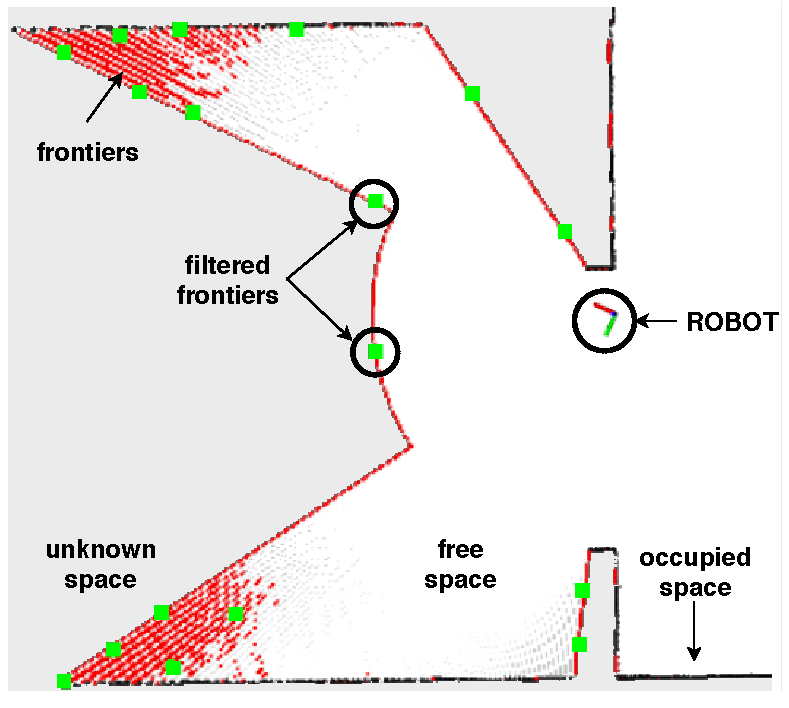
\includegraphics[width=1.0\columnwidth]{./pictures/rviz_environment.pdf}}
	\caption {The environment is represented by a 2D map, with an occupancy grid that divides the map into cells: white cells describe free while grey cells unknown space. Black cells define occupied space (obstacles). Frontiers (red) and filtered frontiers (green).}
	\label{fig:environment}
\end{figure}

%\begin{figure}
%	\centering
%	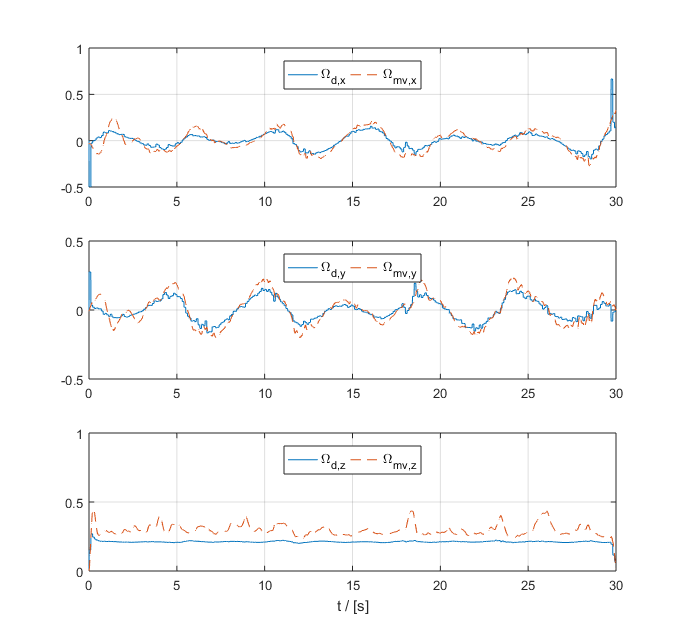
\includegraphics[width=0.85\columnwidth]{./pictures/manip_traj_omega.png}	
%	\caption{Control scheme for the UAV carrying a payload. When considering UAV with MMC \textit{Inverse Jacobian} block becomes the identity matrix. This means that the control inputs $d_x$ and $d_y$ are directly sent as system inputs.}
%	\label{fig:control_scheme}
%\end{figure}

%Zadaci: 
%1. abstract
%2. introduction
%3. 2d exploration - subsection jedan o mom - slika
%3. 3d exploration - subsection jedan o fbet - slika
%4. conclusion